% ============================================================
% LAPORAN PRAKTIKUM ALGORITMA DAN PEMROGRAMAN
% Modul 2: Percabangan Bertingkat dan Perulangan Dasar
% Compile dengan pdfLaTeX
% ============================================================

\documentclass[12pt,a4paper]{article}

% ---------- Font sederhana ----------
\usepackage[T1]{fontenc}
\usepackage[utf8]{inputenc}
\usepackage{mathptmx}

% ---------- Tata letak ----------
\usepackage[a4paper,left=3cm,right=2cm,top=2cm,bottom=2cm]{geometry}
\usepackage{setspace}
\setstretch{1.15}
\usepackage{ragged2e}
\justifying
\setlength{\parindent}{1.25cm}
\setlength{\parskip}{0pt}

% ---------- Paket umum ----------
\usepackage{graphicx}
\usepackage{float}
\usepackage{enumitem}
\usepackage{titlesec}
\usepackage{array}
\usepackage{booktabs}
\usepackage{longtable}
\usepackage{caption}
\usepackage{hyperref}
\usepackage{amsmath}
\hypersetup{hidelinks}

% ---------- Format heading ----------
\titleformat{\section}
  {\bfseries\fontsize{12pt}{14pt}\selectfont}
  {}{0pt}{}
\titlespacing*{\section}{0pt}{12pt}{6pt}

\titleformat{\subsection}
  {\bfseries\fontsize{12pt}{14pt}\selectfont}
  {}{0pt}{}
\titlespacing*{\subsection}{0pt}{10pt}{4pt}

\titleformat{\subsubsection}
  {\bfseries\fontsize{12pt}{14pt}\selectfont}
  {}{0pt}{}
\titlespacing*{\subsubsection}{0pt}{8pt}{3pt}

\setlist[enumerate]{leftmargin=1.1cm,itemsep=0pt,topsep=2pt}
\setlist[itemize]{leftmargin=1.1cm,itemsep=0pt,topsep=2pt}

% ---------- Helper template ----------
\newcommand{\placeholder}[1]{\textit{[#1]}}
\newcommand{\imageplaceholder}[1]{%
  \begin{center}
  \fbox{\parbox[c][5.5cm][c]{0.88\textwidth}{\centering\textit{[#1]}}}
  \end{center}
}

\begin{document}

% ============================================================
% COVER
% ============================================================
\begin{titlepage}
\thispagestyle{empty}
\begin{center}

{\bfseries\fontsize{16pt}{19pt}\selectfont LAPORAN PRAKTIKUM\par}
\vspace{0.25cm}
{\bfseries\fontsize{16pt}{19pt}\selectfont ALGORITMA DAN PEMROGRAMAN\par}
\vspace{0.45cm}
{\bfseries\fontsize{14pt}{17pt}\selectfont MODUL 2\par}
\vspace{0.15cm}
{\bfseries\fontsize{14pt}{17pt}\selectfont PERCABANGAN BERTINGKAT DAN PERULANGAN DASAR\par}

\vspace{1.2cm}

\IfFileExists{logo_telkom_university.png}{%
  
\includegraphics[width=0.34\textwidth]{logo_telkom_university.png}%
}{%
  \IfFileExists{../logo_telkom_university.png}{%
    \includegraphics[width=0.34\textwidth]{../logo_telkom_university.png}%
  }{%
    \IfFileExists{../../logo_telkom_university.png}{%
      
\includegraphics[width=0.34\textwidth]{../../logo_telkom_university.png}%
    }{%
      \fbox{\parbox[c][3.5cm][c]{0.34\textwidth}{\centering\textit{[Logo Telkom University]}}}%
    }%
  }%
}

\vspace{1.2cm}

\renewcommand{\arraystretch}{1.35}
\begin{tabular}{>{\bfseries}p{2.3cm} p{0.35cm} p{8.4cm}}
NAMA  & : & DENDRA DE TAMA \\
NIM   & : & 108052600034 \\
KELAS & : & SS1SI-50-REG-01 \\
PRODI & : & S1 SISTEM INFORMASI \\
\end{tabular}

\vfill

{\bfseries TELKOM UNIVERSITY SURABAYA\par}
{\bfseries FAKULTAS REKAYASA INDUSTRI\par}
{\bfseries PROGRAM STUDI S1 SISTEM INFORMASI\par}
\vspace{0.2cm}
{\bfseries TAHUN AKADEMIK 2025/2026\par}

\end{center}
\end{titlepage}

% ============================================================
% PENDAHULUAN
% ============================================================
\section{PENDAHULUAN}
Struktur kontrol merupakan pilar fundamental dalam perancangan algoritma komputer yang memungkinkan kendali dinamis terhadap alur eksekusi instruksi. Setelah memahami struktur kontrol percabangan sederhana pada Modul 1, penyelesaian masalah komputasi dunia nyata kerap kali menuntut pemodelan logika keputusan yang lebih kompleks dan hierarkis, serta pemrosesan data secara berulang. Modul 2 ini berfokus pada dua konsep esensial dalam Python 3, yaitu percabangan bertingkat (\textit{nested if}) dan struktur perulangan dasar (\textit{looping}).

Percabangan bertingkat (\textit{nested if}) adalah konstruksi logika di mana suatu struktur percabangan diletakkan di dalam blok percabangan lainnya. Mekanisme ini diterapkan ketika suatu keputusan lanjutan hanya relevan untuk dievaluasi apabila kondisi pada tingkat sebelumnya telah terpenuhi. Tingkat kedalaman percabangan dalam Python diatur secara ketat melalui aturan indentasi blok. Pendekatan ini memungkinkan penyaringan kondisi berlapis secara bertahap, seperti pengujian kelayakan usia primer yang dilanjutkan dengan pemeriksaan kepemilikan kartu identitas sekunder untuk penentuan tarif.

Selain logika seleksi berlapis, efisiensi komputasi sangat bergantung pada kemampuan program mengeksekusi sekumpulan instruksi secara berulang tanpa menulis ulang kode sumber. Python menyediakan dua jenis struktur perulangan utama:
\begin{enumerate}
    \item \textbf{Perulangan Terhitung (\textit{Count-Controlled Loop} / \texttt{for})}: Digunakan ketika jumlah iterasi telah diketahui atau ditentukan sebelumnya berdasarkan barisan terurut. Perulangan \texttt{for} pada Python bekerja secara natural melalui mekanisme iterasi objek koleksi dan fungsi pembangun deret bilangan bawaan, yaitu \texttt{range(start, stop, step)}. Parameter \texttt{stop} bersifat eksklusif, sehingga interval yang dihasilkan adalah $[start, stop - 1]$.
    \item \textbf{Perulangan Bersyarat (\textit{Condition-Controlled Loop} / \texttt{while})}: Digunakan ketika perulangan harus terus berlangsung selama suatu kondisi logika bernilai benar (\textit{True}) dan terminasi bergantung pada perubahan status selama eksekusi. Struktur ini sangat ideal untuk menangani perulangan berbasis nilai penanda (\textit{sentinel-controlled loop}), di mana iterasi berhenti ketika masukan khusus diterima, serta sebagai penjaga validitas masukan (\textit{input validation guard}).
\end{enumerate}

Untuk mengendalikan alur iterasi secara fleksibel, Python menyediakan instruksi pengontrol loncatan:
\begin{itemize}
    \item \texttt{break}: Berfungsi menghentikan eksekusi perulangan secara paksa seketika dan langsung memindahkan kendali program ke baris instruksi setelah blok perulangan terdekat.
    \item \texttt{continue}: Berfungsi mengabaikan sisa instruksi pada siklus iterasi yang sedang aktif dan langsung melompat ke evaluasi kondisi iterasi berikutnya.
\end{itemize}

Praktikum Modul 2 ini mencakup empat latihan terarah dan satu studi kasus integratif. Latihan mencakup validasi tiket film 17+ dengan diskon kartu pelajar (\texttt{latihan1.py}), perulangan enumerasi dan tabel perkalian linear (\texttt{latihan2.py}), kalkulator penjumlahan berkelanjutan berbasis nilai sentinel nol (\texttt{latihan3.py}), filter bilangan ganjil dengan terminasi dini (\texttt{latihan4.py}), serta sistem komprehensif rekapitulasi nilai kuis kelas (\texttt{studi\_kasus.py}).

\subsection{Tujuan Praktikum}
\begin{enumerate}
    \item Memahami konsep, sintaksis, dan alur evaluasi percabangan bertingkat (\textit{nested if}) dalam menyelesaikan persoalan keputusan hierarkis.
    \item Mengimplementasikan perulangan terhitung menggunakan struktur \texttt{for} dan fungsi pembangkit deret \texttt{range()}.
    \item Menerapkan perulangan bersyarat \texttt{while} untuk pemrosesan berbasis nilai penanda (\textit{sentinel value}) serta validasi masukan data (\textit{input guard pattern}).
    \item Menganalisis perilaku dan dampak instruksi pengontrol aliran perulangan \texttt{break} dan \texttt{continue} pada alur kerja perulangan.
    \item Merancang solusi terintegrasi yang menggabungkan validasi masukan, perulangan bertingkat, akumulasi data, dan penentuan nilai ekstrem pada studi kasus akademik.
\end{enumerate}

% ============================================================
% LANGKAH PERCOBAAN
% ============================================================
\section{LANGKAH--LANGKAH PERCOBAAN}

\subsection{Percobaan 1: Percabangan Bertingkat Validasi Tiket Bioskop (latihan1.py)}
\begin{enumerate}
    \item Pemahaman Persoalan: Program memvalidasi batasan usia penonton bioskop untuk film kategori usia 17 tahun ke atas. Apabila usia penonton memenuhi syarat ($\ge 17$), program melakukan evaluasi tingkat kedua terhadap status kepemilikan kartu pelajar untuk menentukan harga tiket: Rp30.000 bagi pelajar dan Rp45.000 untuk harga umum. Jika usia kurang dari 17 tahun, akses menonton ditolak secara langsung.
    \item Data Masukan/Keluaran:
    \begin{itemize}
        \item Masukan: Nilai usia pengguna (\texttt{umur}) berupa bilangan bulat integer dan teks status kepemilikan kartu pelajar (\texttt{kartu\_pelajar}) berupa string (\texttt{"ya"} atau \texttt{"tidak"}).
        \item Keluaran: Notifikasi kelayakan usia dan informasi penetapan tarif tiket film, atau pesan penolakan akses masuk.
    \end{itemize}
    \item Penyusunan Algoritma:
    \begin{enumerate}[label=\alph*.]
        \item Mulai program.
        \item Baca masukan usia pengguna, konversi ke tipe integer, dan simpan ke variabel \texttt{umur}.
        \item Baca string masukan konfirmasi kartu pelajar ke variabel \texttt{kartu\_pelajar}.
        \item Evaluasi kondisi luar: jika $umur \ge 17$:
        \begin{enumerate}[label=\roman*.]
            \item Cetak pesan kelayakan: \texttt{"Umur memenuhi syarat nonton film 17+"}.
            \item Evaluasi kondisi dalam: jika $kartu\_pelajar == \text{"ya"}$:
            \begin{itemize}
                \item Cetak \texttt{"Tiket: harga pelajar Rp30000"}.
            \end{itemize}
            \item Selain itu:
            \begin{itemize}
                \item Cetak \texttt{"Tiket: harga umum Rp45000"}.
            \end{itemize}
        \end{enumerate}
        \item Jika $umur < 17$, jalankan blok alternatif luar:
        \begin{itemize}
            \item Cetak pesan penolakan: \texttt{"Maaf, film ini khusus usia 17 tahun ke atas"}.
        \end{itemize}
        \item Selesai.
    \end{enumerate}
\end{enumerate}

\subsection{Percobaan 2: Perulangan for dan Generator range() (latihan2.py)}
\begin{enumerate}
    \item Pemahaman Persoalan: Program mendemonstrasikan dua skenario penggunaan perulangan terhitung (\texttt{for}) dengan bantuan generator interval nilai bawaan \texttt{range(1, 6)}. Skenario pertama melakukan pencacahan sederhana bilangan dari 1 hingga 5. Skenario kedua membuat tabel perkalian linear konstanta 3 dikalikan dengan variabel pencacah deret.
    \item Data Masukan/Keluaran:
    \begin{itemize}
        \item Masukan: Tidak ada masukan dinamis pengguna (deret dihasilkan melalui konstanta kode).
        \item Keluaran: Barisan teks pencacahan nilai 1 sampai 5 serta lima baris perhitungan tabel perkalian konstanta 3 ($3 \times 1$ hingga $3 \times 5$).
    \end{itemize}
    \item Penyusunan Algoritma:
    \begin{enumerate}[label=\alph*.]
        \item Mulai program.
        \item Tampilkan judul bagian pertama: \texttt{"Menghitung dari 1 sampai 5"}.
        \item Inisialisasi perulangan \texttt{for} dengan variabel kontrol \texttt{i} yang melintasi barisan \texttt{range(1, 6)}:
        \begin{itemize}
            \item Cetak string \texttt{"Angka:"} diikuti nilai \texttt{i}.
        \end{itemize}
        \item Cetak satu baris kosong sebagai pemisah visual.
        \item Tampilkan judul bagian kedua: \texttt{"Tabel perkalian 3"}.
        \item Inisialisasi perulangan \texttt{for} kedua dengan variabel kontrol \texttt{i} pada rentang \texttt{range(1, 6)}:
        \begin{itemize}
            \item Hitung hasil perkalian $3 \times i$ dan cetak dalam format \texttt{"3 x [i] = [3*i]"}.
        \end{itemize}
        \item Selesai.
    \end{enumerate}
\end{enumerate}

\subsection{Percobaan 3: Perulangan while Berbasis Nilai Sentinel (latihan3.py)}
\begin{enumerate}
    \item Pemahaman Persoalan: Program berfungsi menghitung akumulasi penjumlahan bilangan bulat yang dimasukkan oleh pengguna secara interaktif. Karena jumlah data masukan tidak dapat dipastikan di awal, program memanfaatkan perulangan \texttt{while} bersyarat dengan menggunakan nilai $0$ sebagai penanda penghentian iterasi (\textit{sentinel value}).
    \item Data Masukan/Keluaran:
    \begin{itemize}
        \item Masukan: Deretan bilangan bulat integer yang dimasukkan pengguna secara bertahap hingga diakhiri dengan input angka 0.
        \item Keluaran: Teks rekapitulasi jumlah total keseluruhan bilangan yang telah diakumulasikan.
    \end{itemize}
    \item Penyusunan Algoritma:
    \begin{enumerate}[label=\alph*.]
        \item Mulai program.
        \item Inisialisasi variabel akumulator \texttt{total} dengan nilai 0.
        \item Baca masukan bilangan bulat pertama dari pengguna ke variabel \texttt{angka}.
        \item Lakukan pengujian kondisi perulangan: selama $angka \ne 0$:
        \begin{enumerate}[label=\roman*.]
            \item Akumulasikan nilai: $total = total + angka$.
            \item Minta dan baca kembali masukan bilangan bulat berikutnya ke variabel \texttt{angka}.
        \end{enumerate}
        \item Setelah perulangan terhenti (saat pengguna memasukkan 0), cetak teks \texttt{"Total semua angka: "} diikuti nilai variabel \texttt{total}.
        \item Selesai.
    \end{enumerate}
\end{enumerate}

\subsection{Percobaan 4: Pengendalian Iterasi dengan break dan continue (latihan4.py)}
\begin{enumerate}
    \item Pemahaman Persoalan: Program menguji manipulasi alur kontrol perulangan terhitung \texttt{for} pada interval bilangan 1 sampai 10. Program menerapkan instruksi \texttt{continue} untuk melompati proses pencetakan saat variabel iterasi bernilai genap, serta menerapkan instruksi \texttt{break} untuk menghentikan seluruh proses perulangan seketika begitu variabel iterasi mencapai angka 8.
    \item Data Masukan/Keluaran:
    \begin{itemize}
        \item Masukan: Tidak ada masukan dinamis (menggunakan deret bilangan 1 sampai 10).
        \item Keluaran: Teks judul, barisan bilangan ganjil yang lolos penyaringan sebelum angka 8 (1, 3, 5, 7), dan notifikasi penutup perulangan.
    \end{itemize}
    \item Penyusunan Algoritma:
    \begin{enumerate}[label=\alph*.]
        \item Mulai program.
        \item Cetak informasi judul proses.
        \item Inisialisasi perulangan \texttt{for} dengan variabel \texttt{i} pada rentang \texttt{range(1, 11)}:
        \begin{enumerate}[label=\roman*.]
            \item Uji kondisi terminasi dini: jika $i == 8$, jalankan instruksi \texttt{break} untuk keluar dari blok perulangan.
            \item Uji kondisi paritas: jika $i \pmod 2 == 0$, jalankan instruksi \texttt{continue} untuk langsung melompat ke iterasi berikutnya tanpa mengeksekusi baris bawahnya.
            \item Tampilkan nilai \texttt{i}.
        \end{enumerate}
        \item Cetak teks penutup: \texttt{"Perulangan selesai"}.
        \item Selesai.
    \end{enumerate}
\end{enumerate}

\subsection{Percobaan 5: Studi Kasus Rekapitulasi Nilai Kuis Kelas (studi\_kasus.py)}
\begin{enumerate}
    \item Pemahaman Persoalan: Program mengintegrasikan seluruh teknik perulangan dan percabangan bertingkat untuk membangun sistem rekapitulasi nilai kuis akademik satu kelas. Program membaca jumlah mahasiswa, melakukan validasi ketat agar nilai kuis berada pada rentang valid $0 \le nilai \le 100$ menggunakan perulangan \texttt{while}, mengklasifikasikan kategori capaian menggunakan percabangan bertingkat (\textit{nested if}), menghitung akumulasi total nilai, menentukan nilai ekstrem (tertinggi dan terendah), serta mencetak ringkasan statistik kelas.
    \item Data Masukan/Keluaran:
    \begin{itemize}
        \item Masukan: Bilangan bulat jumlah mahasiswa (\texttt{jumlah\_mahasiswa}) dan nilai kuis numerik untuk setiap mahasiswa.
        \item Keluaran: Kategori capaian mahasiswa per individu (\texttt{"Lulus Sangat Baik"}, \texttt{"Lulus"}, \texttt{"Remedial"}, atau \texttt{"Tidak Lulus"}), serta ringkasan rekapitulasi kuis (nilai rata-rata berformat satu desimal, nilai tertinggi, nilai terendah, jumlah mahasiswa lulus, remedial, dan tidak lulus).
    \end{itemize}
    \item Penyusunan Algoritma:
    \begin{enumerate}[label=\alph*.]
        \item Mulai program.
        \item Inisialisasi variabel statistik: $total = 0$, $lulus = 0$, $remedial = 0$, $tidak\_lulus = 0$, $tertinggi = 0$, dan $terendah = \text{None}$.
        \item Baca masukan bilangan integer ke dalam variabel \texttt{jumlah\_mahasiswa}.
        \item Inisialisasi perulangan \texttt{for} dengan indeks $i$ mulai dari 1 sampai $jumlah\_mahasiswa$:
        \begin{enumerate}[label=\roman*.]
            \item Baca nilai mahasiswa ke-$i$ ke variabel \texttt{nilai}.
            \item Lakukan validasi masukan dengan perulangan \texttt{while}: selama $nilai < 0$ atau $nilai > 100$, cetak peringatan galat rentang dan minta pengguna memasukkan kembali \texttt{nilai}.
            \item Evaluasi percabangan bertingkat:
            \begin{itemize}
                \item Jika $nilai \ge 60$:
                \begin{itemize}
                    \item Jika $nilai \ge 85$: $kategori = \text{"Lulus Sangat Baik"}$.
                    \item Selain itu: $kategori = \text{"Lulus"}$.
                    \item Tambahkan pencacah kelulusan: $lulus = lulus + 1$.
                \end{itemize}
                \item Selain itu (jika $nilai < 60$):
                \begin{itemize}
                    \item Jika $nilai \ge 40$: $kategori = \text{"Remedial"}$, tambahkan $remedial = remedial + 1$.
                    \item Selain itu: $kategori = \text{"Tidak Lulus"}$, tambahkan $tidak\_lulus = tidak\_lulus + 1$.
                \end{itemize}
            \end{itemize}
            \item Tampilkan kategori capaian mahasiswa ke-$i$.
            \item Akumulasikan total nilai: $total = total + nilai$.
            \item Perbarui nilai tertinggi: jika $nilai > tertinggi$, tetapkan $tertinggi = nilai$.
            \item Perbarui nilai terendah: jika $terendah \text{ is None}$ atau $nilai < terendah$, tetapkan $terendah = nilai$.
        \end{enumerate}
        \item Hitung nilai rata-rata: $rata\_rata = total / jumlah\_mahasiswa$ jika $jumlah\_mahasiswa > 0$, selain itu bernilai 0.
        \item Tampilkan blok rekapitulasi statistik kuis kelas secara terstruktur.
        \item Selesai.
    \end{enumerate}
\end{enumerate}

% ============================================================
% HASIL DAN ANALISIS
% ============================================================
\section{HASIL DAN ANALISIS PERCOBAAN}

Pada bagian ini disajikan algoritma komputasi terperinci, dokumentasi luaran eksekusi program, serta analisis mendalam terhadap lima percobaan praktikum Python 3 pada Modul 2.

\subsection{Percobaan 1: Percabangan Bertingkat Validasi Tiket Bioskop}
\subsubsection{Algoritma}
\begin{enumerate}
    \item Mulai program.
    \item Panggil fungsi \texttt{input("Masukkan umur: ")}, ubah ke bilangan bulat \texttt{int}, dan simpan ke variabel \texttt{umur}.
    \item Panggil fungsi \texttt{input("Punya kartu pelajar? (ya/tidak): ")} dan simpan ke variabel string \texttt{kartu\_pelajar}.
    \item Uji kondisi tingkat pertama: periksa apakah $umur \ge 17$:
    \begin{enumerate}[label=\alph*.]
        \item Jika benar (\textit{True}): cetak \texttt{"Umur memenuhi syarat nonton film 17+"}.
        \begin{enumerate}[label=\roman*.]
            \item Uji kondisi bertingkat kedua: periksa apakah $kartu\_pelajar == \text{"ya"}$.
            \item Jika benar (\textit{True}): cetak \texttt{"Tiket: harga pelajar Rp30000"}.
            \item Jika salah (\textit{False}): cetak \texttt{"Tiket: harga umum Rp45000"}.
        \end{enumerate}
        \item Jika salah (\textit{False}): langsung alihkan eksekusi ke blok \texttt{else} luar dan cetak teks penolakan \texttt{"Maaf, film ini khusus usia 17 tahun ke atas"}.
    \end{enumerate}
    \item Selesai.
\end{enumerate}

\subsubsection{Hasil / Output}
\begin{figure}[H]
    \centering
    \IfFileExists{image/latihan1.png}{%
        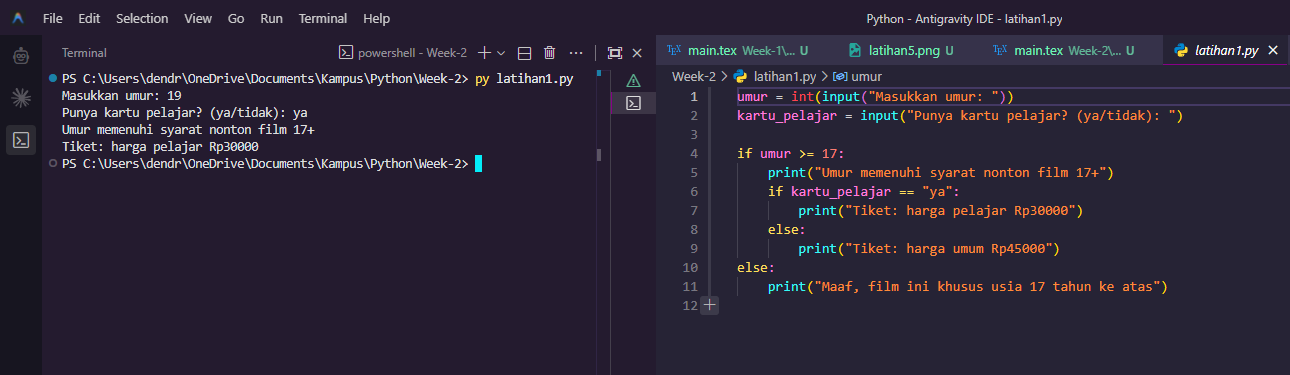
\includegraphics[width=0.85\textwidth]{image/latihan1.png}%
    }{%
        \imageplaceholder{Output Percobaan 1: Percabangan Bertingkat Tiket Bioskop}%
    }
    \caption{Hasil/Output Percobaan 1: Percabangan Bertingkat Tiket Bioskop}
\end{figure}

\subsubsection{Analisis}
Percobaan 1 mendemonstrasikan efisiensi struktur percabangan bertingkat (*nested if*) dalam memodelkan ketergantungan keputusan. Keunggulan dari pola bertingkat ini adalah eliminasi evaluasi redundan; program tidak perlu menguji kepemilikan kartu pelajar apabila syarat primer batasan umur ($umur \ge 17$) tidak terpenuhi.

Secara teknis, interpreter Python mengevaluasi ekspresi pada blok terluar terlebih dahulu. Jika masukan umur adalah 16, kondisi luar bernilai \textit{False}, sehingga seluruh blok instruksi pada tubuh \texttt{if} luar (termasuk percabangan kartu pelajar) diabaikan sepenuhnya dan eksekusi melompat langsung ke blok penolakan \texttt{else} terluar. Sebaliknya, ketika masukan umur adalah 19, kondisi luar bernilai \textit{True}, pesan kelayakan usia dicetak, lalu alur mengevaluasi status string \texttt{kartu\_pelajar}. Apabila bernilai \texttt{"ya"}, tarif diskon pelajar Rp30.000 diterapkan; selain itu tarif standar umum Rp45.000 yang berlaku. Hal ini membuktikan keteraturan hierarki alur keputusan berbasis indentasi spasi pada Python.

\subsection{Percobaan 2: Perulangan for dan Generator range()}
\subsubsection{Algoritma}
\begin{enumerate}
    \item Mulai program.
    \item Cetak string pembuka \texttt{"Menghitung dari 1 sampai 5"}.
    \item Jalankan perulangan \texttt{for} dengan variabel penunjuk \texttt{i} pada rentang \texttt{range(1, 6)}:
    \begin{enumerate}[label=\alph*.]
        \item Cetak teks \texttt{"Angka:"} dan nilai \texttt{i} yang dipisahkan spasi.
    \end{enumerate}
    \item Cetak satu baris kosong menggunakan pemanggilan fungsi \texttt{print()} tanpa argumen.
    \item Cetak string judul kedua \texttt{"Tabel perkalian 3"}.
    \item Jalankan perulangan \texttt{for} kedua dengan variabel penunjuk \texttt{i} pada rentang \texttt{range(1, 6)}:
    \begin{enumerate}[label=\alph*.]
        \item Hitung ekspresi $3 \times i$ dan cetak \texttt{"3 x", i, "=", 3 * i}.
    \end{enumerate}
    \item Selesai.
\end{enumerate}

\subsubsection{Hasil / Output}
\begin{figure}[H]
    \centering
    \IfFileExists{image/latihan2.png}{%
        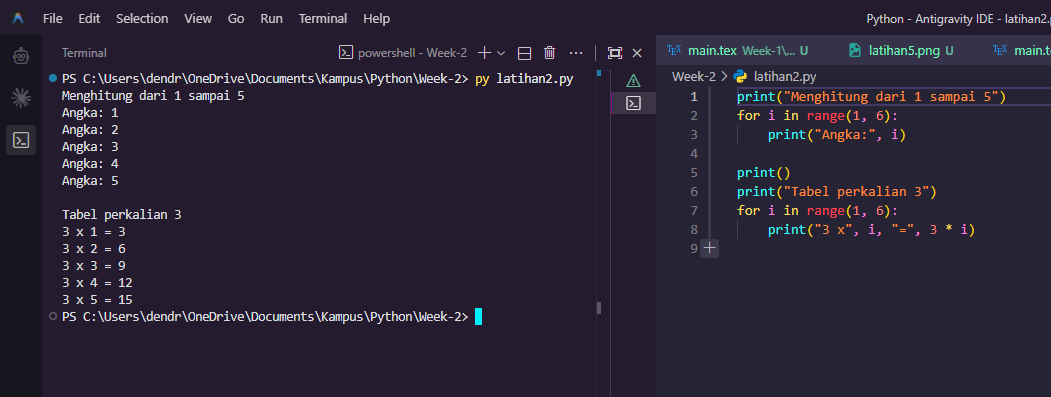
\includegraphics[width=0.85\textwidth]{image/latihan2.png}%
    }{%
        \imageplaceholder{Output Percobaan 2: Perulangan for dan range()}%
    }
    \caption{Hasil/Output Percobaan 2: Perulangan for dan range()}
\end{figure}

\subsubsection{Analisis}
Percobaan 2 memperlihatkan pemanfaatan perulangan terhitung (*count-controlled loop*) menggunakan kata kunci \texttt{for} yang dipadukan dengan fungsi bawaan \texttt{range()}. Objek yang dihasilkan oleh \texttt{range(start, stop)} adalah generator bilangan bulat semi-terbuka $[start, stop)$, yang berarti batas akhir bersifat eksklusif. Oleh karena itu, \texttt{range(1, 6)} membangkitkan barisan bilangan 1, 2, 3, 4, dan 5 secara berurutan tepat sebanyak 5 siklus iterasi.

Pada bagian tabel perkalian, variabel iterasi \texttt{i} bertindak sebagai pengali variabel independen terhadap konstanta 3. Di setiap iterasi, ekspresi $3 * i$ dievaluasi secara dinamis menghasilkan nilai 3, 6, 9, 12, dan 15. Penggunaan fungsi \texttt{print()} dengan multi-argumen secara implisit menggabungkan parameter dengan spasi tunggal, menghasilkan luaran tabel aritmatika yang seragam dan mudah dibaca tanpa memerlukan konkatenasi string manual.

\subsection{Percobaan 3: Perulangan while Berbasis Nilai Sentinel}
\subsubsection{Algoritma}
\begin{enumerate}
    \item Mulai program.
    \item Inisialisasi variabel penyimpan hasil akumulasi: tetapkan $total = 0$.
    \item Lakukan pembacaan masukan nilai awal (\textit{priming read}): baca teks masukan, ubah menjadi integer, dan simpan ke variabel \texttt{angka}.
    \item Uji kondisi perulangan \texttt{while}: selama $angka \ne 0$:
    \begin{enumerate}[label=\alph*.]
        \item Tambahkan nilai masukan ke dalam akumulator: $total = total + angka$.
        \item Baca masukan berikutnya dari konsol ke variabel \texttt{angka} untuk dievaluasi pada siklus selanjutnya.
    \end{enumerate}
    \item Tampilkan hasil akumulasi akhir: \texttt{"Total semua angka: "} diikuti nilai variabel \texttt{total}.
    \item Selesai.
\end{enumerate}

\subsubsection{Hasil / Output}
\begin{figure}[H]
    \centering
    \IfFileExists{image/latihan3.png}{%
        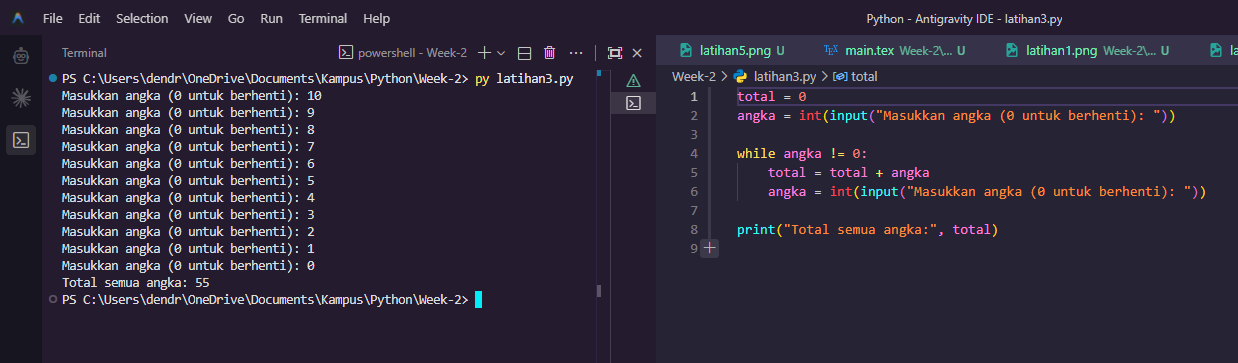
\includegraphics[width=0.85\textwidth]{image/latihan3.png}%
    }{%
        \imageplaceholder{Output Percobaan 3: Perulangan while Berbasis Nilai Sentinel}%
    }
    \caption{Hasil/Output Percobaan 3: Perulangan while Berbasis Nilai Sentinel}
\end{figure}

\subsubsection{Analisis}
Percobaan 3 mengimplementasikan perulangan bersyarat (*condition-controlled loop*) dengan pola nilai penanda (*sentinel-controlled loop*). Berbeda dengan \texttt{for} loop yang jumlah siklusnya statis, perulangan \texttt{while} mengevaluasi ekspresi logika $angka \ne 0$ sebelum setiap iterasi dimulai. Iterasi akan terus berulang selama nilai variabel \texttt{angka} bukan nol.

Pola pembacaan masukan awal sebelum blok perulangan (\textit{priming read}) dan pembacaan ulang di akhir badan perulangan merupakan kaidah baku perancangan algoritma sentinel. Langkah ini memastikan bahwa nilai sentinel itu sendiri (angka 0) tidak ikut terakumulasi ke dalam variabel \texttt{total}, karena begitu nilai 0 dimasukkan, kondisi perulangan seketika bernilai \textit{False} dan alur keluar dari perulangan. Mekanisme ini menjamin integritas kalkulasi matematis akumulator.

\subsection{Percobaan 4: Pengendalian Iterasi dengan break dan continue}
\subsubsection{Algoritma}
\begin{enumerate}
    \item Mulai program.
    \item Cetak informasi judul program deret ganjil.
    \item Jalankan perulangan \texttt{for} dengan variabel penunjuk deret \texttt{i} pada interval \texttt{range(1, 11)}:
    \begin{enumerate}[label=\alph*.]
        \item Evaluasi kondisi pemutus: periksa apakah $i == 8$.
        \begin{itemize}
            \item Jika benar (\textit{True}): eksekusi perintah \texttt{break} untuk menolak dan menghentikan seluruh perulangan.
        \end{itemize}
        \item Evaluasi kondisi filter paritas: periksa apakah sisa bagi genap $i \pmod 2 == 0$.
        \begin{itemize}
            \item Jika benar (\textit{True}): eksekusi perintah \texttt{continue} untuk mengabaikan eksekusi pencetakan dan langsung melompat ke iterasi $i$ berikutnya.
        \end{itemize}
        \item Tampilkan nilai variabel \texttt{i} ke konsol.
    \end{enumerate}
    \item Cetak pesan konfirmasi penghentian: \texttt{"Perulangan selesai"}.
    \item Selesai.
\end{enumerate}

\subsubsection{Hasil / Output}
\begin{figure}[H]
    \centering
    \IfFileExists{image/latihan4.png}{%
        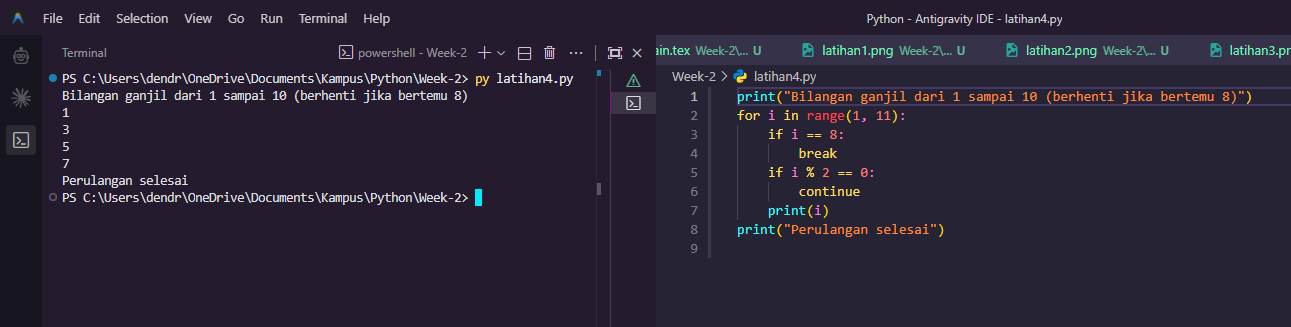
\includegraphics[width=0.85\textwidth]{image/latihan4.png}%
    }{%
        \imageplaceholder{Output Percobaan 4: Pengendalian Iterasi break dan continue}%
    }
    \caption{Hasil/Output Percobaan 4: Pengendalian Iterasi break dan continue}
\end{figure}

\subsubsection{Analisis}
Percobaan 4 membuktikan secara empiris perbedaan mendasar antara instruksi pengontrol loncatan \texttt{break} dan \texttt{continue}:
\begin{itemize}
    \item Pada saat $i$ bernilai genap (2, 4, 6), kondisi $i \pmod 2 == 0$ terpenuhi, sehingga instruksi \texttt{continue} dieksekusi. Perintah ini menghentikan siklus iterasi yang sedang aktif dan seketika melompat ke iterasi berikutnya, sehingga instruksi \texttt{print(i)} di bawahnya terlewati. Hasilnya, angka genap tersaring keluar dari tampilan konsol.
    \item Pada saat $i$ mencapai nilai 8, kondisi $i == 8$ bernilai \textit{True}, sehingga instruksi \texttt{break} dieksekusi. Berbeda dengan \texttt{continue}, \texttt{break} menghentikan perulangan \texttt{for} secara permanen. Akibatnya, nilai-nilai berikutnya (8, 9, dan 10) tidak pernah diproses sama sekali.
\end{itemize}
Kombinasi kedua kata kunci tersebut menghasilkan deret luaran yang terpotong rapi hanya pada angka ganjil 1, 3, 5, dan 7 sebelum diakhiri dengan pencetakan teks \texttt{"Perulangan selesai"}.

\subsection{Percobaan 5: Studi Kasus Rekapitulasi Nilai Kuis Kelas}
\subsubsection{Algoritma}
\begin{enumerate}
    \item Mulai program.
    \item Alokasikan dan inisialisasi variabel statistik: $total = 0$, $lulus = 0$, $remedial = 0$, $tidak\_lulus = 0$, $tertinggi = 0$, serta $terendah = \text{None}$.
    \item Baca masukan bilangan bulat ke dalam variabel \texttt{jumlah\_mahasiswa}.
    \item Lakukan perulangan terhitung \texttt{for} dengan indeks $i$ mulai dari 1 sampai $jumlah\_mahasiswa$:
    \begin{enumerate}[label=\alph*.]
        \item Baca nilai ujian mahasiswa ke-$i$ ke variabel \texttt{nilai}.
        \item Masuk ke blok perlindungan validasi (\textit{input guard}): selama $nilai < 0$ atau $nilai > 100$, cetak notifikasi \texttt{"Nilai harus 0-100, coba lagi"} dan baca ulang masukan ke variabel \texttt{nilai}.
        \item Evaluasi hierarki capaian nilai:
        \begin{itemize}
            \item Jika $nilai \ge 60$:
            \begin{itemize}
                \item Jika $nilai \ge 85$: tetapkan $kategori = \text{"Lulus Sangat Baik"}$.
                \item Selain itu: tetapkan $kategori = \text{"Lulus"}$.
                \item Tambahkan pencacah kelulusan: $lulus = lulus + 1$.
            \end{itemize}
            \item Selain itu (apabila $nilai < 60$):
            \begin{itemize}
                \item Jika $nilai \ge 40$: tetapkan $kategori = \text{"Remedial"}$ dan perbarui $remedial = remedial + 1$.
                \item Selain itu: tetapkan $kategori = \text{"Tidak Lulus"}$ dan perbarui $tidak\_lulus = tidak\_lulus + 1$.
            \end{itemize}
        \end{itemize}
        \item Tampilkan teks kategori capaian: \texttt{f"Kategori: \{kategori\}"}.
        \item Akumulasikan nilai: $total = total + nilai$.
        \item Perbarui batas nilai tertinggi: jika $nilai > tertinggi$, simpan $tertinggi = nilai$.
        \item Perbarui batas nilai terendah: jika $terendah \text{ is None}$ atau $nilai < terendah$, simpan $terendah = nilai$.
    \end{enumerate}
    \item Evaluasi nilai rata-rata kelas secara aman terhadap potensi galat pembagian dengan nol (\textit{zero division guard}): jika $jumlah\_mahasiswa > 0$ maka $rata\_rata = total / jumlah\_mahasiswa$, selain itu 0.
    \item Tampilkan blok rekapitulasi data kuis: cetak nilai rata-rata dengan pembulatan satu digit di belakang koma (\texttt{.1f}), nilai tertinggi, nilai terendah, serta jumlah mahasiswa pada masing-masing kategori kelulusan.
    \item Selesai.
\end{enumerate}

\subsubsection{Hasil / Output}
\begin{figure}[H]
    \centering
    \IfFileExists{image/studi_kasus.png}{%
        \includegraphics[width=0.85\textwidth]{image/studi_kasus.png}%
    }{%
        \IfFileExists{image/latihan5.png}{%
            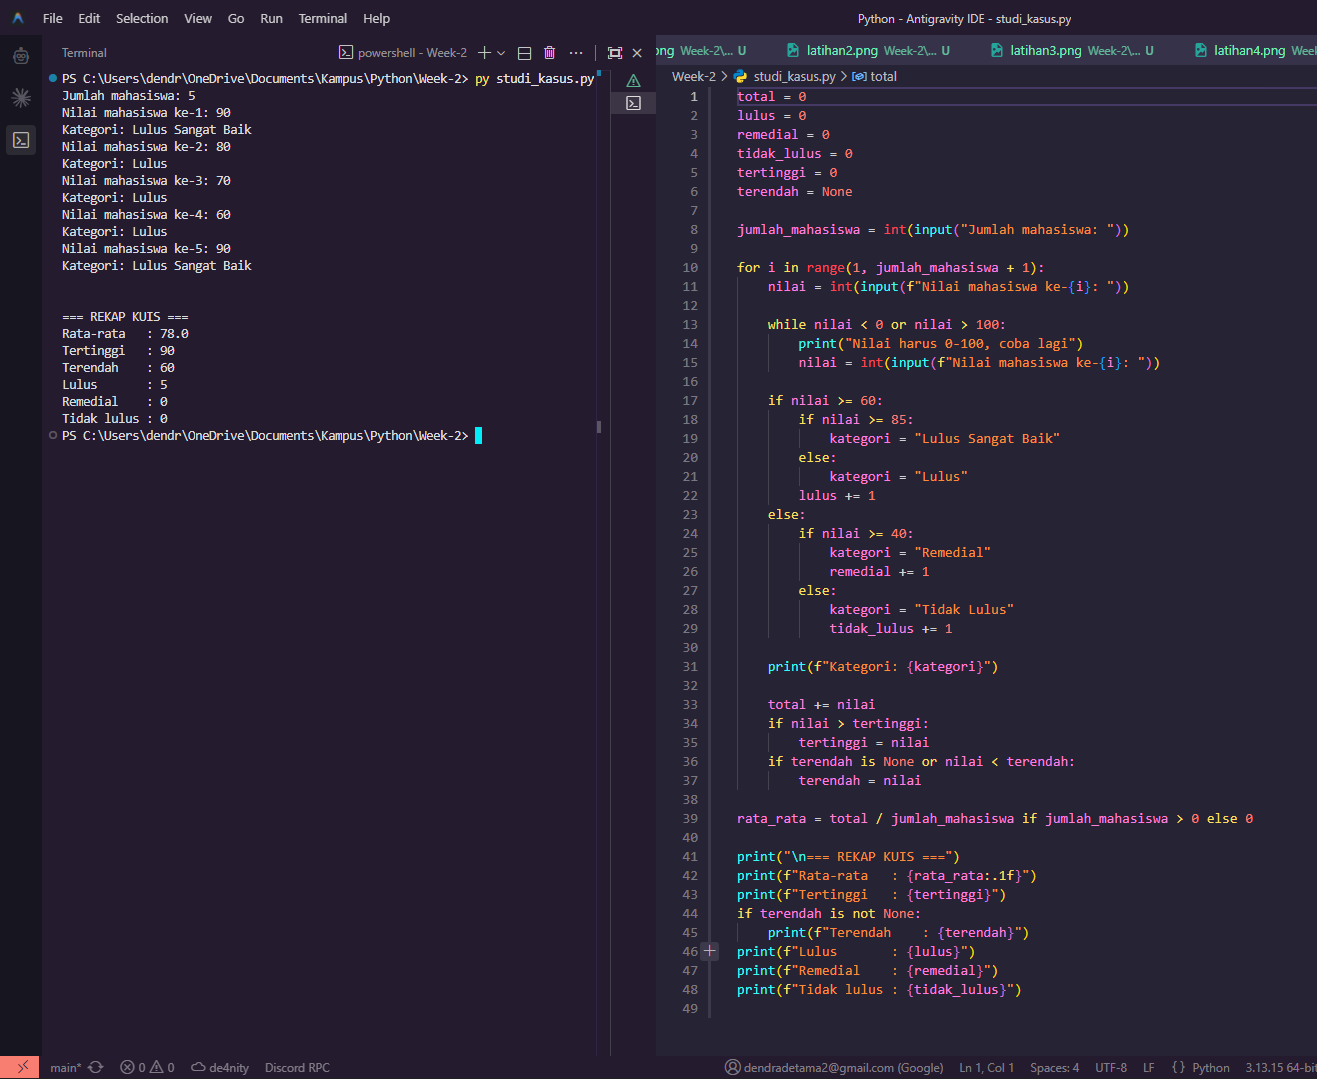
\includegraphics[width=0.85\textwidth]{image/latihan5.png}%
        }{%
            \imageplaceholder{Output Percobaan 5: Studi Kasus Rekapitulasi Nilai Kuis Kelas}%
        }%
    }
    \caption{Hasil/Output Percobaan 5: Studi Kasus Rekapitulasi Nilai Kuis Kelas}
\end{figure}

\subsubsection{Analisis}
Studi kasus ini merepresentasikan arsitektur pemrosesan data batch sederhana berbasis konsol. Program memadukan empat teknik algoritmik fundamental:
\begin{enumerate}
    \item \textbf{Validasi Masukan (\textit{Input Guard Pattern})}: Penggunaan \texttt{while nilai < 0 or nilai > 100} mengisolasi data anomali sebelum diproses. Pengguna dipaksa memasukkan data ulang secara kontinu hingga masukan berada dalam interval tertutup $[0, 100]$. Hal ini menjaga kekokohan (*robustness*) sistem terhadap kesalahan manusia (*human error*).
    \item \textbf{Klasifikasi Bertingkat (\textit{Hierarchical Classification})}: Logika penentuan kategori memisahkan domain lulus ($\ge 60$) dan tidak lulus ($< 60$) pada tingkat pertama, sebelum memperincinya ke predikat spesifik (85 untuk Sangat Baik dan 40 untuk Remedial). Pendekatan modular ini memudahkan pemeliharaan kode dan penambahan kategori baru di masa mendatang.
    \item \textbf{Penentuan Nilai Ekstrem Dinamis}: Inisialisasi $terendah = \text{None}$ merupakan praktik terbaik (*best practice*) dalam Python. Jika $terendah$ diinisialisasi dengan angka nol, maka data mahasiswa dengan nilai valid di atas nol (misalnya nilai terendah 50) tidak akan pernah menggantikan nilai awal nol tersebut. Dengan membandingkan $terendah \text{ is None}$ pada iterasi pertama, nilai awal mahasiswa pertama secara otomatis menjadi patokan awal perbandingan.
    \item \textbf{Agregasi dan Format Output}: Penggunaan ekspresi kondisional ternari satu baris (\textit{ternary operator}) pada perhitungan rata-rata mencegah galat fatal \texttt{ZeroDivisionError} apabila masukan jumlah mahasiswa adalah 0. Pemformatan ekspresi \texttt{\{rata\_rata:.1f\}} memastikan nilai presisi mengambang ditampilkan secara bersih dengan satu desimal.
\end{enumerate}

% ============================================================
% KESIMPULAN
% ============================================================
\section{KESIMPULAN}
Berdasarkan serangkaian percobaan dan implementasi yang dilakukan pada Praktikum Modul 2, ditarik beberapa kesimpulan sebagai berikut:
\begin{enumerate}
    \item Percabangan bertingkat (\textit{nested if}) menyediakan mekanisme penanganan logika keputusan hierarkis berlapis yang efisien dengan mengeliminasi pengujian syarat sekunder yang tidak relevan apabila syarat primer tidak terpenuhi.
    \item Perulangan \texttt{for} bersama fungsi pembangkit interval \texttt{range()} sangat efektif untuk mengotomasi proses iterasi dengan jumlah siklus terhitung (*count-controlled loop*), dengan karakteristik batas akhir interval yang bersifat eksklusif ($[start, stop)$).
    \item Perulangan bersyarat \texttt{while} memberikan fleksibilitas tinggi dalam menangani proses iterasi yang jumlah eksekusinya tidak dapat diprediksi secara apriori, seperti akumulasi berbasis penanda (*sentinel*) serta penyaringan validasi data masukan konsol (*input guard*).
    \item Kata kunci \texttt{break} dan \texttt{continue} memberikan kendali tingkat lanjut terhadap aliran iterasi; \texttt{break} menghentikan perulangan sepenuhnya secara seketika, sedangkan \texttt{continue} hanya mengabaikan sisa instruksi pada siklus saat ini dan melompat ke siklus iterasi berikutnya.
    \item Penggunaan nilai penanda awal \texttt{None} pada pelacakan nilai minimum dinamis dan pencegahan galat pembagian nol (\textit{zero division guard}) merupakan prinsip rekayasa perangkat lunak esensial dalam menghasilkan program komputasi yang tangguh (*robust*) dan andal.
\end{enumerate}

% ============================================================
% DAFTAR PUSTAKA
% ============================================================
\section{DAFTAR PUSTAKA}

\begin{enumerate}
    \item Tim Dosen Algoritma dan Pemrograman. (2025). \textit{Modul Praktikum 2: Percabangan Bertingkat dan Perulangan Dasar}. Program Studi S1 Sistem Informasi, Fakultas Rekayasa Industri, Telkom University Surabaya.

    \item Python Software Foundation. (2024). \textit{Python Language Reference: Compound Statements (Release 3.12)}. Diakses dari \url{https://docs.python.org/3/reference/compound_stmts.html}.

    \item Downey, A. (2015). \textit{Think Python: How to Think Like a Computer Scientist (2nd Edition)}. O'Reilly Media.
\end{enumerate}

\end{document}
